\documentclass[xcolor={dvipsnames},aspectratio=169,10pt]{beamer}

% utility packages
\usepackage{multicol}
\usepackage{relsize}
\usepackage{amsthm}
\usepackage[spanish]{babel}
\usepackage{biblatex}
\usepackage{fontawesome}
\usepackage{pgfplots}
\usepackage{enumitem}
\usepackage{empheq}
\usepackage{xcolor}
\usepackage{epigraph}

% better text justifying
\usepackage{microtype}
% justify text inside list environment
% Ref: http://liam0205.me/2017/04/11/justifying-in-beamer-s-lists/
\usepackage{ragged2e}
\makeatletter
\patchcmd{\itemize}{\raggedright}{\justifying}{}{}
\patchcmd{\beamer@enum@}{\raggedright}{\justifying}{}{}
\patchcmd{\@@description}{\raggedright}{\justifying}{}{}
\makeatother

% math related packages
\usepackage{amsmath}
\usepackage[ruled,vlined]{algorithm2e}
\SetAlCapNameFnt{\scriptsize}
\SetAlCapFnt{\scriptsize}
\SetAlFnt{\scriptsize}

% figure related packages
\usepackage{graphicx}
\usepackage[scale=2]{ccicons}
\usepackage{tikz}
\usepackage{tikzpagenodes}
\usetikzlibrary{decorations.pathreplacing}
\usetikzlibrary{positioning}

% table related packages
\usepackage{array}
\usepackage{booktabs}
\usepackage{multirow}
\usepackage{colortbl}
\newcommand{\tabincell}[2]{\begin{tabular}{@{}#1@{}}#2\end{tabular}}

% hyperref setting
\hypersetup{
  unicode,
  psdextra,
  bookmarksnumbered=true,
  bookmarksopen=true,
  bookmarksopenlevel=3,
  bookmarksdepth=4,
  pdfcenterwindow=true,
  pdfstartview={Fit},
  pdfpagemode={FullScreen},
  pdfpagelayout={SinglePage},
}
\usepackage{bookmark}

% beamer theme
\usetheme{metropolis}
\metroset{block=fill,numbering=fraction}

% caption style
\usepackage{subcaption}
\setlength\abovecaptionskip{3pt}
\setbeamerfont{caption}{size=\scriptsize}
\renewcommand{\figurename}{Fig.}
\captionsetup{labelformat=empty,labelsep=none,textfont={bf,it}}

% Ref: https://github.com/gpoore/minted/blob/master/source/minted.dtx
\newenvironment{latexexample}
{\VerbatimEnvironment\begin{VerbatimOut}[gobble=3]{example.out}}{\end{VerbatimOut}%
  \begin{center}
    \begin{minipage}{0.47\linewidth}%
      \inputminted[resetmargins,fontsize=\scriptsize]{latex}{example.out}%
    \end{minipage}%
    \hspace{0.05\linewidth}%
    \begin{minipage}{0.47\linewidth}%
      \begin{framed}
        \setlength{\parindent}{2em}%
        \input{example.out}%
      \end{framed}
    \end{minipage}%
  \end{center}
}

\newenvironment{mathexample}
{\VerbatimEnvironment\begin{VerbatimOut}[gobble=3]{example.out}}{\end{VerbatimOut}%
  \begin{center}
    \begin{minipage}{0.47\linewidth}%
      \inputminted[resetmargins,fontsize=\scriptsize]{latex}{example.out}%
    \end{minipage}%
    \hspace{0.05\linewidth}%
    \begin{minipage}{0.47\linewidth}%
      \begin{framed}
        \[ \input{example.out} \]
      \end{framed}
    \end{minipage}%
  \end{center}
}

\newenvironment{mathexamples}
{\VerbatimEnvironment\begin{VerbatimOut}[gobble=3]{example.out}}{\end{VerbatimOut}%
  \begin{center}
    \begin{minipage}{0.47\linewidth}%
      \inputminted[resetmargins,fontsize=\scriptsize]{latex}{example.out}%
    \end{minipage}%
    \hspace{0.05\linewidth}%
    \begin{minipage}{0.47\linewidth}%
      \begin{framed}
        \directlua{
          local first = true
          for line in io.lines('example.out') do
          if first then
          first = false
          else
          tex.print('\\newline ')
          end
          tex.print('$' .. line .. '$')
          end
        }
      \end{framed}
    \end{minipage}%
  \end{center}
}
\begin{document}

\title{Obtención de los Coeficientes de la forma canónica para la Elipse, hipérbolas y parábolas}
\subtitle{Determinación analítica de las cónicas}
\author{Grupo 8}
\date{December 05, 2023}
\titlegraphic{
  \begin{tikzpicture}[overlay, remember picture]
    \node[%
      above right=0.35cm and -0.2cm of current page footer area.south west,
      anchor=south west,
      inner sep=0pt] {%
      \usebeamerfont{footline}
    };
    % \node[%
    %   above left=0.35cm and 0cm of current page footer area.south east,
    %   anchor=south east,
    %   inner sep=0pt]{\qrcode[height=1.5cm]{https://github.com/axvg/presentaciones}};
  \end{tikzpicture}
}

\maketitle%

\begin{frame}
\epigraph{``Sigue intentando. Sigue intentando. Incurre en todos los errores posibles. Simplemente sigue intentando''}{-René Descartes}
\end{frame}

\begin{frame}{Contenidos}
  \setbeamertemplate{section in toc}[sections numbered]
  \tableofcontents[hideallsubsections]
\end{frame}

\section{Introducción}

\begin{frame}{Formas cuadráticas}
    \frametitle{Formas cuadráticas}
    \begin{block}{Definición}
      Una forma cuadrática en n variables $x_{1}, x_{2}, . . . , x_{n}$ es una combinación lineal de los
      productos $x_{i} x_{j}$, esto es, una combinación lineal de cuadrados $x_{1}^2 , x_{2}^2 , . . . , x_{n}^2$ y
      términos $x_{1}x_{2}, x_{1}x_{3}, . . . , x_{1}x_{n}, x_{2}x_{3}, . . . , x_{2}x_{n}, . . . , x_{n-1}x_{n}$
    \end{block}

  \begin{block}{Ejemplos}
    \begin{itemize}
        \item $q = x^2 - y^2 + 4xy$ y $q = x^2 + 3y^2 - 2xy$ son formas cuadráticas en $x$ y $y$.
        \item $q = -4x_{21} + x_{22}^2 + 4x_{23} + 6x_{1}x_{3}$ es una forma cuadrática en $x_{1}, x_{2}$ y $x_{3}$.
        \item La forma cuadrática general de $x_{1}, x_{2}, x_{3}$ es $a_{1}x_{21} + a_{2}x_{22}^2 + a_{3}x_{23} + a_{12}x_{1}x_{2} + a_{13}x_{1}x_{3} + a_{23}x_{2}x_{3}$.
    \end{itemize}
  \end{block}
\end{frame}

\begin{frame}{Formas cuadráticas}
  \frametitle{Formas cuadráticas}
  Las formas cuadráticas pueden ser escritas de la forma matricial $q(x) = x^{T}Ax$ donde $A$ es una matriz simétrica $n 
  \times n$ y $x$ es un vector columna $n \times 1$.

  La matriz $A$ es llamada la matriz de la forma cuadrática $q$.

  \begin{block}{Ejemplos}
    Supongamos que $q = x_1^2 - x_2^2 + 4x_1x_2$. Los coeficientes de $x_1^2$ y $x_2^2$ son 1 y -1, 
    respectivamente, por lo que colocamos estos, en orden, en las dos posiciones diagonales de una matriz A. 
    El coeficiente de $x_1x_2$ es 4, que dividimos equitativamente entre las posiciones (1, 2) y (2, 1), 
    colocando un 2 en cada lugar.
  \end{block}
\end{frame}

\begin{frame}{Formas cuadráticas}
  \frametitle{Formas cuadráticas}
  Así tenemos que:
  \begin{equation*}
    A = \begin{bmatrix}
      1 & 2 \\
      2 & -1
    \end{bmatrix}
  \end{equation*}
  y $x = \begin{bmatrix}
    x_1 \\
    x_2
  \end{bmatrix}$.
  Luego:
  \begin{equation*}
    q(x) = x^{T}Ax = \begin{bmatrix}
      x_1 & x_2
    \end{bmatrix}
    \begin{bmatrix}
      1 & 2 \\
      2 & -1
    \end{bmatrix}
    \begin{bmatrix}
      x_1 \\
      x_2
    \end{bmatrix}
    = x_1^2 - x_2^2 + 4x_1x_2
  \end{equation*}
\end{frame}

\section{Secciones Cónicas}

\begin{frame}{Secciones Cónicas}
  \frametitle{Secciones Cónicas}
  Se utiliza el término cónica para referirse a todas las curvas que surgen de las diversas intersecciones entre un cono y un plano. 
  Cuando dicho plano no cruza el vértice, se generan las cónicas específicas: parábola, elipse, hipérbola y circunferencia. 
  En este proyecto, nos enfocaremos únicamente en las tres primeras. 
  \begin{figure}
    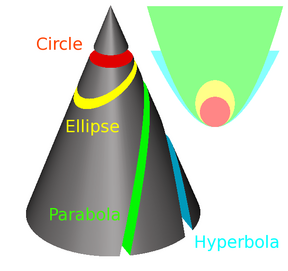
\includegraphics[width=0.5\textwidth, height=0.6\textheight, keepaspectratio]{images/conics.png}
    \caption{Las secciones cónicas: círculo, elipse, parábola y hipérbola}
  \end{figure}
\end{frame}

\begin{frame}{Forma General de las Secciones Cónicas}
  \begin{definition}
    Una sección cónica es el lugar en el plano cartesiano $\mathbb{R}^2$ de una ecuación de la forma
    \begin{equation*}
      ax^2 + bxy + cy^2 + dx + ey + f = 0. \tag{1}
    \end{equation*}
  \end{definition}
  Se puede demostrar que esta ecuación representa uno de los siguientes:
  \begin{itemize}
    \item El conjunto vacío.
    \item Un solo punto.
    \item Una o dos rectas.
    \item Una elipse.
    \item Una hipérbola.
    \item Una parábola.
\end{itemize}
  La parte de segundo grado de (1), $q(x, y) = ax^2 + bxy + cy^2$ es una forma cuadrática. Esto determina el tipo de la cónica.
\end{frame}

\begin{frame}{Forma Matricial de las Secciones Cónicas}
  \frametitle{Forma Matricial de las Secciones Cónicas}
  Podemos escribir la ecuación en forma matricial:
  \begin{equation*}
    [x, y] \begin{bmatrix} a & b/2 \\ b/2 & c \end{bmatrix} \begin{bmatrix} x \\ y \end{bmatrix} + [d, e] \begin{bmatrix} x \\ y \end{bmatrix} + f = 0.
  \end{equation*}
  Escribimos $A = \begin{bmatrix} a & b/2 \\ b/2 & c \end{bmatrix}$. Sea $U = [u, v]$ una matriz ortogonal cuyos vectores de columna $u$ y $v$ son vectores propios de $A$ con valores propios $\lambda_1$ y $\lambda_2$. Aplicamos el cambio de variables
  \begin{equation*}
    x = \begin{bmatrix} x \\ y \end{bmatrix} = U \begin{bmatrix} u \\ v \end{bmatrix}
  \end{equation*}
  para diagonalizar la forma cuadrática $q(x, y)$ a la forma diagonal
  \begin{equation*}
    \lambda_1u^2 + \lambda_2v^2.
  \end{equation*}
\end{frame}

\begin{frame}{Transformación de Coordenadas}
  \frametitle{Transformación de Coordenadas}
  La base ortonormal \{u, v\} determina un nuevo conjunto de ejes de coordenadas con respecto a los cuales el lugar de la ecuación
  \begin{equation*}
    [x, y] A [x, y]^T + B [x, y]^T + f = 0
  \end{equation*}
  con B = [d, e] es el mismo que el lugar de la ecuación
  \begin{equation*}
    0 = [u, v] \text{diag} (\lambda_1, \lambda_2) [u, v]^T + (BU) [u, v]^T + f
  \end{equation*}
  por lo tanto
  \begin{equation*}
    \lambda_1 u^2 + \lambda_2 v^2 + [d, e] [u, v] [u, v]^T + f = 0 \tag{2}
  \end{equation*}
\end{frame}

\begin{frame}{Determinación del Tipo de Cónica}
  \frametitle{Determinación del Tipo de Cónica}
  Si la cónica determinada por (2) no es degenerada, es decir, no es un conjunto vacío, un punto, ni línea(s), entonces los signos de $\lambda_1$ y $\lambda_2$ determinan si es una parábola, una hipérbola o una elipse. La ecuación (1) representará
  \begin{itemize}
    \item una elipse si $\lambda_1\lambda_2 > 0$,
    \item una hipérbola si $\lambda_1\lambda_2 < 0$,
    \item una parábola si $\lambda_1\lambda_2 = 0$.
  \end{itemize}
\end{frame}

\section{Forma reducida de las Secciones Cónicas}
\begin{frame}{Idea para clasificar cónicas}
  \frametitle{Idea para clasificar cónicas}
  
  \begin{columns}
    \column{0.4\textwidth}
    Ecuación en la referencia inicial:
    \begin{equation*}
      a_{11}x^2 + 2a_{12}xy + a_{22}y^2 + 2a_{13}x + 2a_{23}y + a_{33} = 0
    \end{equation*}
    \begin{equation*}
      A = \begin{bmatrix}
        a_{11} & a_{12} & a_{13} \\
        a_{12} & a_{22} & a_{23} \\
        a_{13} & a_{23} & a_{33}
      \end{bmatrix}
    \end{equation*}

    \column{0.2\textwidth}
    \begin{center}
      \begin{tikzpicture}
        \draw[->] (0,0) -- (1,0);
      \end{tikzpicture}
    \end{center}

    \column{0.4\textwidth}
    Ecuación en la nueva referencia:
    \begin{equation*}
      \lambda_1x'^2 + \lambda_2y'^2 + d= 0
    \end{equation*}

    \begin{equation*}
      A' = \begin{bmatrix}
        \lambda_1 & 0 & 0 \\
        0 & \lambda_2 & 0 \\
        0 & 0 & d
      \end{bmatrix}
    \end{equation*}
  \end{columns}
\end{frame}

\begin{frame}{Idea para clasificar cónicas}
  \frametitle{Idea para clasificar cónicas}
  \begin{figure}
    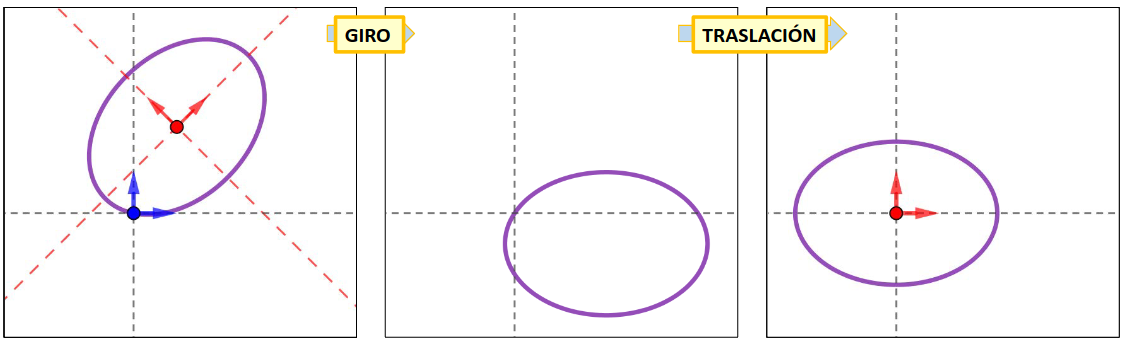
\includegraphics[width=\textwidth, height=\textheight, keepaspectratio]{images/red.png}
  \end{figure}
\end{frame}

\begin{frame}{Giro o eliminación del término cruzado - Parte 1}
  \frametitle{Giro o eliminación del término cruzado}
  Cónica en la referencia inicial:
  \begin{equation*}
    a_{11}x^2 + \textcolor{red}{2a_{12}xy} + a_{22}y^2 + 2a_{13}x + 2a_{23}y + a_{33} = 0
  \end{equation*}
  \begin{equation*}
    \begin{pmatrix} x & y \end{pmatrix} T \begin{pmatrix} x \\ y \end{pmatrix} + 2\begin{pmatrix} a_{13} & a_{23} \end{pmatrix} \begin{pmatrix} x \\ y \end{pmatrix} + a_{33} = 0
  \end{equation*}
  
  \begin{block}{Teorema}
    \begin{equation*}
      T \text{ es simétrica } \Rightarrow \exists P \text{ tal que } P^{-1} = P^T \text{ y } P^T T P = D = \begin{bmatrix} \lambda_1 & 0 \\ 0 & \lambda_2 \end{bmatrix} \text{ es diagonal}    
    \end{equation*}
  \end{block}
\end{frame}

\begin{frame}{Giro o eliminación del término cruzado - Parte 2}
  Cambio de referencia:
  \begin{equation*}
    \begin{pmatrix} x \\ y \end{pmatrix} = P \begin{pmatrix} x' \\ y' \end{pmatrix}
  \end{equation*}

  \begin{equation*}
    \begin{pmatrix} x' & y' \end{pmatrix} P^T T P \begin{pmatrix} x' \\ y' \end{pmatrix} + 2\begin{pmatrix} a_{13} & a_{23} \end{pmatrix} P \begin{pmatrix} x' \\ y' \end{pmatrix} + a_{33} = 0
  \end{equation*}
  
  \begin{equation*}
    \begin{pmatrix} x' & y' \end{pmatrix} D \begin{pmatrix} x' \\ y' \end{pmatrix} + 2\begin{pmatrix} a_{13} & a_{23} \end{pmatrix} P \begin{pmatrix} x' \\ y' \end{pmatrix} + a_{33} = 0
  \end{equation*}

  Cónica en nueva referencia:
  \begin{equation*}
    \boxed{\lambda_1x'^2 + \lambda_2y'^2 + 2b_{13}x' + 2b_{23}y' + a_{33} = 0}
  \end{equation*}
\end{frame}

\begin{frame}{Traslación o eliminación de la parte lineal - Parte 1}
  \frametitle{Traslación o eliminación de la parte lineal}
  Ecuacion hasta ahora:
  \begin{equation*}
    \boxed{\lambda_1x'^2 + \lambda_2y'^2 + \textcolor{red}{2b_{13}x'} + \textcolor{red}{2b_{23}y'} + a_{33} = 0}
  \end{equation*}

  Completando cuadrados:
  \begin{equation*}
    \lambda_{1}x'^2 + 2b_{13}x' = \lambda_{1}\left(x' - \frac{b_{13}}{\lambda_{1}}\right)^2 - \frac{b_{13}^2}{\lambda_{1}}
  \end{equation*}
  
  \begin{equation*}
    \lambda_{2}y'^2 + 2b_{23}y' = \lambda_{2}\left(y' - \frac{b_{23}}{\lambda_{2}}\right)^2 - \frac{b_{23}^2}{\lambda_{2}}
  \end{equation*}

  Reemplazando en la ecuación:
  \begin{equation*}
    \boxed{\lambda_{1}\left(x' - \frac{b_{13}}{\lambda_{1}}\right)^2 + \lambda_{2}\left(y' - \frac{b_{23}}{\lambda_{2}}\right)^2 + a_{33} - \frac{b_{13}^2}{\lambda_{1}} - \frac{b_{23}^2}{\lambda_{2}} = 0}
  \end{equation*}

\end{frame}

\begin{frame}{Traslación o eliminación de la parte lineal - Parte 2}
  \frametitle{Traslación o eliminación de la parte lineal}

  Cambio de referencia (traslación):
  \begin{equation*}
    \begin{pmatrix} x'' \\ y'' \end{pmatrix} = \begin{pmatrix} x' \\ y' \end{pmatrix} - \begin{pmatrix} \frac{b_{13}}{2\lambda_{1}} \\ \frac{b_{23}}{2\lambda_{2}} \end{pmatrix}
  \end{equation*}

  \begin{equation*}
    \lambda_{1}x''+ \lambda_{2}y'' - \frac{b_{23}^2}{\lambda_{2}}  - \frac{b_{13}^2}{\lambda_{1}}  + a_{33} = 0
  \end{equation*}

  \begin{equation*}
    \colorbox{yellow}{$\displaystyle\lambda_{1}x''^2 + \lambda_{2}y''^2 + d = 0$}
  \end{equation*}
\end{frame}

\begin{frame}{Clasificación}
  \frametitle{Clasificación}
  \begin{table}[]
    \begin{tabular}{|c|c|c|c|}
    \hline
    & $|A| > 0$ & $|A| = 0$ & $|A| < 0$ \\ \hline
    $T > 0$ & Elipse imaginaria & Rectas imaginarias cortándose & Elipse real \\ \hline
    $T = 0$ & Parábola, $rg(A) = 2$ & $\begin{aligned} &\text{rg(A) = 2} \\ &\{\text{Rectas paralelas imag.} \\ &\text{Rectas paralelas reales}\} \\ &\text{rg(A) = 1 Recta doble} \end{aligned}$ & Recta doble, Parábola \\ \hline
    $T < 0$ & Hipérbola & Rectas reales cortándose & Hipérbola \\ \hline
    \end{tabular}
  \end{table}
\end{frame}

\begin{frame}{Parábola}
  \frametitle{Parábola}
  Una parábola es el lugar geométrico de un punto que se mueve en un plano de tal manera que su distancia a una recta fija, llamada directriz, situada en el mismo plano, 
  es siempre igual a su distancia a un punto fijo del plano, llamado foco, y que no pertenece a la recta.

  \begin{columns}
    \begin{column}{0.5\textwidth}
      \begin{figure}
        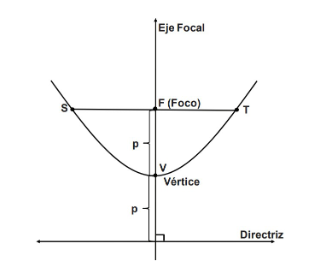
\includegraphics[width=\textwidth, height=0.6\textheight, keepaspectratio]{images/par1.png}
        \caption{Parábola y elementos}
      \end{figure}
    \end{column}
    \begin{column}{0.5\textwidth}
      \begin{itemize}\small
        \itemsep0em
        \item Eje Focal: es la recta que pasa por el foco y el vértice
        \item Foco (F): es el punto fijo que se indica en la definición
        \item Directriz: es la recta fija mencionada en la definición
        \item Vértice (V): es el punto donde el eje focal corta la parábola
        \item Distancia focal (p): es la distancia desde el vértice al foco y del vértice a la directriz.
        \item Lado Recto (ST): es el segmento perpendicular al eje focal, que pasa por el foco F, cuyos extremos son dos puntos de la parábola.
      \end{itemize}
    \end{column}
  \end{columns}
\end{frame}

\begin{frame}{Parámetros de la Parábola}
  \frametitle{Parámetros de la Parábola}

  \begin{table}[]
    \begin{tabular}{|c|c|c|}
    \hline
    & Parábola de eje vertical & Parábola de eje horizontal \\ \hline
    Ecuación General & $Ax^2 + Dx + Ey + F = 0$ & $Cy^2 + Dx + Ey + F = 0$ \\ 
    & $C = 0, A\neq0$ & $A = 0, C\neq 0$ \\ \hline
    Ecuación canónica & $(x-h)^2 = 4p(y-k)$ & $(y-k)^2 = 4p(x-h)$ \\ \hline
    Coordenadas del Vértice & $(h, k)$ & $(h, k)$ \\ \hline
    Coordenadas del Foco & $(h, k+p)$ & $(h+p, k)$ \\ \hline
    Ecuación de la Directriz & $y=k-p$ & $x=h-p$ \\ \hline
    Ecuación del eje focal & $x=h$ & $y=k$ \\ \hline
    \end{tabular}
  \end{table}
\end{frame}

\begin{frame}{Ecuaciones reducidas, foco, directriz y excentricidad de la parábola - Parte 1}
  \frametitle{Ecuaciones reducidas, foco, directriz y excentricidad de la parábola - Parte 1}
    Ecuación reducida de la parábola:
    \[\lambda_1x'^2 - 2dy' = 0\]
    con $\lambda_1$ autovalor no nulo de T y $d = +\sqrt{-\frac{det(A)}{\lambda_1}}$.
    
    Ecuación de cambio de referencia:
    \[\begin{pmatrix} x \\ y \end{pmatrix} = \begin{pmatrix} \text{vertice} \end{pmatrix} + \begin{pmatrix} \text{autovec1} \\ \text{autovec2} \end{pmatrix} \begin{pmatrix} x' \\ y' \end{pmatrix}.\]
  \end{frame}

\begin{frame}{Ecuaciones reducidas, foco, directriz y excentricidad de la parábola - Parte 2}
  \frametitle{Ecuaciones reducidas, foco, directriz y excentricidad de la parábola - Parte 2}
    Hay que orientar el autovector asociado al 0 de forma que $\begin{pmatrix} a_{13} & a_{23} \end{pmatrix} \begin{pmatrix} \text{autovec2} \end{pmatrix} < 0$.
    
    Ecuación canónica:
    \[x'^2 = 2py'\]
    
    Foco en nueva referencia: $F' = (0, \frac{p}{2})$.
    
    Foco en referencia inicial: Se aplica la ecuación de cambio de referencia a $F'$.
    
    Directriz: Recta polar del foco $F = (s, t)$: $\begin{pmatrix} s & t & 1 \end{pmatrix} \begin{pmatrix} x \\ y \\ 1 \end{pmatrix} = 0$
    
    Excentricidad: $e = 1$
\end{frame}

\begin{frame}{Elipse}
  \frametitle{Elipse}
    Una elipse es el conjunto de todos los puntos en un plano cuya distancia a dos puntos fijos en el plano tienen una suma constante. 
    Los puntos fijos son los focos de la elipse. La recta que une los focos es el eje focal. El punto sobre el eje focal que está en el 
    punto medio entre los dos focos es el centro. Los puntos donde la elipse interseca a su eje son los vértices de la elipse.
  \begin{columns}
    \begin{column}{0.5\textwidth}
      \begin{figure}
        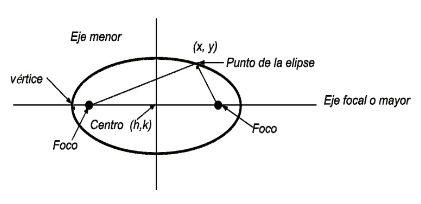
\includegraphics[width=\textwidth, height=0.6\textheight, keepaspectratio]{images/eli1.png}
        \caption{Parábola y elementos}
      \end{figure}
    \end{column}
    \begin{column}{0.5\textwidth}
      \begin{itemize}
        \item Eje Mayor: es el segmento que pasa por los focos y los vértices de la elipse
        \item Eje Menor: es el segmento perpendicular al eje mayor en el centro de la elipse
        \item Focos (F): son los dos puntos fijos en la definición de la elipse
        \item Vértices (V): son los puntos donde el eje mayor corta la elipse
      \end{itemize}
    \end{column}
  \end{columns}
\end{frame}

\begin{frame}{Elementos de la Elipse}
  \frametitle{Elementos de la Elipse}
  \begin{table}[]
    \small
    \begin{tabular}{|c|>{\centering\arraybackslash}p{4cm}|>{\centering\arraybackslash}p{4cm}|}
    \hline
    & Elipse de eje horizontal & Elipse de eje vertical \\ \hline
    Ecuación General & \multicolumn{2}{c|}{$Ax^2 + Cy^2 + Dx + Ey + F = 0$} \\ \hline
    Condiciones & \multicolumn{2}{c|}{\parbox{8cm}{Con $A$ y $C$ no ambas cero, mismo valor numérico. $B = 0$ (Sin rotación de ejes)}} \\ \hline
    Ecuación canónica & \multicolumn{2}{c|}{\rule{0pt}{2.5ex}$\frac{(x-h)^2}{a^2} + \frac{(y-k)^2}{b^2} = 1$} \\ \hline
    Localización de los focos & $(h \pm c, k)$ & $(h, k \pm c)$ \\ \hline
    Localización de los vértices & $(h \pm a, k)$ & $(h, k \pm a)$ \\ \hline
    Ecuación del eje mayor & $y=k$ & $x=h$ \\ \hline
    Semieje mayor & \multicolumn{2}{c|}{$a$} \\ \hline
    Semieje menor & \multicolumn{2}{c|}{$b$} \\ \hline
    Distancia focal & \multicolumn{2}{c|}{$c$} \\ \hline
    Relación pitagórica & \multicolumn{2}{c|}{$c^2 = a^2 - b^2$} \\ \hline
    \end{tabular}
  \end{table}
\end{frame}

\begin{frame}{Ecuaciones reducidas, focos, directrices y excentricidad de la elipse - Parte 1}
  \frametitle{Ecuaciones reducidas, focos, directrices y excentricidad de la elipse - Parte 1}
    Ecuación reducida de la elipse:
    \[\lambda_1x'^2 + \lambda_2y'^2 + d = 0\]
    con $\lambda_1, \lambda_2 > 0$ autovalores de T, ordenados de forma que $\lambda_2 \geq \lambda_1$ y $d = \frac{det(A)}{det(T)}$.
    
    Ecuación de cambio de referencia:
    \[\begin{pmatrix} x \\ y \end{pmatrix} = \begin{pmatrix} \text{centro} \end{pmatrix} + \begin{pmatrix} \text{autovec1} \\ \text{autovec2} \end{pmatrix} \begin{pmatrix} x' \\ y' \end{pmatrix}.\]
\end{frame}

\begin{frame}{Ecuaciones reducidas, focos, directrices y excentricidad de la elipse - Parte 2}
  \frametitle{Ecuaciones reducidas, focos, directrices y excentricidad de la elipse - Parte 2}
    Ecuación canónica:
    \[\frac{x'^2}{a^2} + \frac{y'^2}{b^2} = 1\]
    
    Focos en nueva referencia: $F'_1 = (c, 0)$ y $F'_2 = (-c, 0)$, con $c = +\sqrt{a^2 - b^2}$.
    
    Focos en referencia inicial: Se aplica la ecuación de cambio de referencia a $F'_1$ y $F'_2$.
    
    Directrices: Rectas polares de los focos $F_i = (s_i, t_i)$: $\begin{pmatrix} s_i & t_i & 1 \end{pmatrix} \begin{pmatrix} x \\ y \\ 1 \end{pmatrix} = 0$
    
    Excentricidad: $e = \frac{c}{a} < 1$
\end{frame}

\begin{frame}{Hipérbola}
  \frametitle{Hipérbola}
    Una hipérbola es el conjunto de todos los puntos en un plano cuya diferencia de distancias a dos puntos fijos en el plano es una constante. 
    Los puntos fijos son los focos de la hipérbola. La recta que une los focos es el eje focal. El punto sobre el eje focal que está en el 
    punto medio entre los dos focos es el centro. Los puntos donde la hipérbola interseca a su eje son los vértices de la hipérbola.
    \begin{columns}
      \begin{column}{0.5\textwidth}
        \begin{figure}
          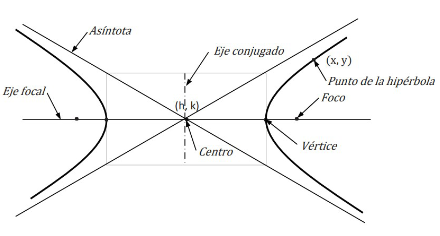
\includegraphics[width=\textwidth, height=0.6\textheight, keepaspectratio]{images/hyp1.png}
          \caption{Parábola y elementos}
        \end{figure}
      \end{column}
      \begin{column}{0.5\textwidth}
        \begin{itemize}
          \item Eje Transverso: es el segmento que pasa por los focos y los vértices de la hipérbola
          \item Eje Conjugado: es el segmento perpendicular al eje transverso en el centro de la hipérbola
          \item Focos (F): son los dos puntos fijos en la definición de la hipérbola
          \item Vértices (V): son los puntos donde el eje transverso corta la hipérbola
        \end{itemize}
      \end{column}
    \end{columns}
\end{frame}

\begin{frame}{Elementos de la Hipérbola}
  \frametitle{Elementos de la Hipérbola}
  \begin{table}[]
    \small
    \begin{tabular}{|c|>{\centering\arraybackslash}p{4cm}|>{\centering\arraybackslash}p{4cm}|}
    \hline
    & Hipérbola de eje horizontal & Hipérbola de eje vertical \\ \hline
    Ecuación General & \multicolumn{2}{c|}{$Ax^2 - Cy^2 + Dx + Ey + F = 0$} \\ \hline
    Condiciones & \multicolumn{2}{c|}{\parbox{8cm}{Con $A$ y $C$ no ambas cero, distinto valor numérico y signos contrarios. $B = 0$ (Sin rotación de ejes)}} \\ \hline
    Ecuación canónica & \multicolumn{2}{c|}{\rule{0pt}{2.5ex}$\frac{(x-h)^2}{a^2} - \frac{(y-k)^2}{b^2} = 1$} \\ \hline
    Localización de los focos & $(h \pm c, k)$ & $(h, k \pm c)$ \\ \hline
    Localización de los vértices & $(h \pm a, k)$ & $(h, k \pm a)$ \\ \hline
    Ecuación del eje focal & $y=k$ & $x=h$ \\ \hline
    Semieje focal & \multicolumn{2}{c|}{$a$} \\ \hline
    Semieje conjugado & \multicolumn{2}{c|}{$b$} \\ \hline
    Longitud focal & \multicolumn{2}{c|}{$c$} \\ \hline
    Relación pitagórica & \multicolumn{2}{c|}{$c^2 = a^2 + b^2$} \\ \hline
    Ecuación de las asinfotas & $y = k \pm \frac{b}{a}(x - h)$ & $x = h \pm \frac{a}{b}(y - k)$ \\ \hline
    \end{tabular}
  \end{table}
\end{frame}

\begin{frame}{Ecuaciones reducidas, focos, directrices y excentricidad de la hipérbola - Parte 1}
  \frametitle{Ecuaciones reducidas, focos, directrices y excentricidad de la hipérbola - Parte 1}
    Ecuación reducida de la hipérbola:
    \[\lambda_1x'^2 + \lambda_2y'^2 + d = 0\]
    con $\lambda_1, \lambda_2$ autovalores de T, ordenados de forma que $signo(\lambda_1) = signo(det(A))$ y $d = \frac{det(A)}{det(T)}$.
    
    Ecuación de cambio de referencia:
    \[\begin{pmatrix} x \\ y \end{pmatrix} = \begin{pmatrix} \text{centro} \end{pmatrix} + \begin{pmatrix} \text{autovec1} \\ \text{autovec2} \end{pmatrix} \begin{pmatrix} x' \\ y' \end{pmatrix}.\]
  \end{frame}

\begin{frame}{Ecuaciones reducidas, focos, directrices y excentricidad de la hipérbola - Parte 2}
  \frametitle{Ecuaciones reducidas, focos, directrices y excentricidad de la hipérbola - Parte 2}
    Ecuación canónica:
    \[\frac{x'^2}{a^2} - \frac{y'^2}{b^2} = 1\]
    
    Focos en nueva referencia: $F'_1 = (c, 0)$ y $F'_2 = (-c, 0)$, con $c = +\sqrt{a^2 + b^2}$.
    
    Focos en referencia inicial: Se aplica la ecuación de cambio de referencia a $F'_1$ y $F'_2$.
    
    Directrices: Rectas polares de los focos $F_i = (s_i, t_i)$: $\begin{pmatrix} s_i & t_i & 1 \end{pmatrix} \begin{pmatrix} x \\ y \\ 1 \end{pmatrix} = 0$
    
    Excentricidad: $e = \frac{c}{a} > 1$
\end{frame}

\section{Ejercicios}
\begin{frame}{Ejercicio 1:}
  \frametitle{Ejercicio 1:}
  \begin{block}{Ejercicio}
    En el plano afín dada la cónica de ecuación:
    \[x^2 - 2xy + y^2 + 4x + 1 = 0\]
    (i) Clasificar la cónica.
  \end{block}
    La matriz asociada a la cónica y de términos cuadráticos son respectivamente:
    \[A = \begin{pmatrix} 1 & -1 & 2 \\ -1 & 1 & 0 \\ 2 & 0 & 1 \end{pmatrix}, T = \begin{pmatrix} 1 & -1 \\ -1 & 1 \end{pmatrix}.\]
    Se tiene que det(A) = -4 y det(T) = 0. Se trata por tanto de una parábola.
\end{frame}

\begin{frame}{Ejercicio 1: (Continuación)}
  \frametitle{Ejercicio 1: (Continuación)}
    (ii) Hallar su centro, ejes, vértices y asíntotas.
    Dado que es una parábola, no tiene ni centro ni asíntotas.
    El eje es la línea polar del autovector asociado al autovalor no nulo de T.
    El polinomio característico de T es:
    \[|T - \lambda Id| = (1 - \lambda)^2 - 1^2 = \lambda^2 - 2\lambda = \lambda(\lambda - 2).\]
    Por lo tanto, el autovalor no nulo es $\lambda_1 = 2$. Sus autovectores asociados verifican
    \[(T - 2Id) \begin{pmatrix} x \\ y \end{pmatrix} = \begin{pmatrix} 0 \\ 0 \end{pmatrix} \Leftrightarrow -x - y = 0\]
    Por lo tanto, $S_2 = L\{(1, -1)\}$.
    El eje será la línea polar del vector (1, -1):
    \[(1, -1, 0) A \begin{pmatrix} x \\ y \\ 1 \end{pmatrix} = 0 \Leftrightarrow 2x - 2y + 2 = 0 \Leftrightarrow x - y + 1 = 0.\]
\end{frame}

\begin{frame}{Ejercicio 1: (Continuación)}
  \frametitle{Ejercicio 1: (Continuación)}
    (iii) Calcular su ecuación reducida, excentricidad y distancia del vértice al foco.
    Por ser una parábola la excentricidad es e = 1.
    La ecuación reducida es de la forma:
    \[\lambda_1x''^2 - 2cy'' = 0 \Leftrightarrow 2x''^2 - 2cy'' = 0,\]
    donde
    \[c = \sqrt{-\frac{|A|}{\lambda_1}} = \sqrt{2}.\]
    La ecuación reducida queda:
    \[x''^2 - \sqrt{2}y'' = 0. (*)\]
\end{frame}

\begin{frame}{Ejercicio 1: (Continuación)}
  \frametitle{Ejercicio 1: (Continuación)}
    Ahora sabemos que cuando está expresada de la forma $x^2 = 2py$ el foco está en el punto $(0, p/2)$ y el vértice en el origen. Por tanto la distancia focal es $p/2$. En nuestro caso si reescribimos:
    \[x''^2 - \frac{2\sqrt{2}}{2}y'' = 0,\]
    vemos que $p = \sqrt{2}/2$ y así la distancia del vértice al foco es $p/2 = \sqrt{2}/4$.
\end{frame}

% \begin{frame}{Ejercicio 2: (Continuación)}
%   \frametitle{Ejercicio 2: (Continuación)}
%   \begin{block}{Ejercicio}
%   Para cada número real a definimos la cónica de ecuación:
%   \[9x^2 + ay^2 - 6axy + 3a - 12 = 0.\]
%   (i) Clasificar las cónicas dependiendo de los valores de a.
%   \end{block}
%   La matriz asociada a la cónica y de términos cuadráticos son respectivamente:
%   \[A = \begin{pmatrix} 9 & -3a & 0 \\ -3a & a & 0 \\ 0 & 0 & 3a - 12 \end{pmatrix}, T = \begin{pmatrix} 9 & -3a \\ -3a & a \end{pmatrix}.\]
%   Vemos que:
%   \[|A| = (3a - 12)(9a - 9a^2) = 27a(a - 4)(1 - a), |T| = 9a - 9a^2 = 9a(1 - a).\]
%   Los puntos donde se anulan son a = 0, 1, 4. Estudiamos los siguientes casos:
% \end{frame}

% \begin{frame}{Ejercicio 2: (Continuación)}
%   \frametitle{Ejercicio 2: (Continuación)}
%   \begin{enumerate}[label=(\roman*)]
%     \item $a < 0$. Se tiene que $|T| < 0$ y $|A| > 0$. Se trata de una hipérbola.
%     \item $a = 0$. Se tiene que $|T| = 0$ y $|A| = 0$. Se trata de rectas paralelas reales o imaginarias o coincidentes.
%   \end{enumerate}
%   En particular la ecuación queda:
%   \[9x^2 - 12 = 0 \Leftrightarrow (3x - \sqrt{12})(3x + \sqrt{12}) = 0.\]
%   Es decir se tratan de rectas paralelas reales.
% \end{frame}

% \begin{frame}{Ejercicio 2: (Continuación)}
%   \frametitle{Ejercicio 2: (Continuación)}
%   \begin{enumerate}[label=(\roman*),start=3]
%     \item $0 < a < 1$. Se tiene que $|T| > 0$ y $|A| < 0$. Se trata de una elipse real.
%     \item $a = 1$. Se tiene que $|T| = 0$ y $|A| = 0$. Se trata de rectas paralelas reales o imaginarias o coincidentes.
%   \end{enumerate}
%   La matriz asociada queda:
%   \[A = \begin{pmatrix} 9 & -3 & 0 \\ -3 & 1 & 0 \\ 0 & 0 & -9 \end{pmatrix}.\]
%   Haciendo congruencia:
%   \[A = \begin{pmatrix} 9 & -3 & 0 \\ -3 & 1 & 0 \\ 0 & 0 & -9 \end{pmatrix} \rightarrow \begin{pmatrix} 9 & 0 & 0 \\ 0 & 0 & 0 \\ 0 & 0 & -9 \end{pmatrix}\]
%   y vemos que de nuevo se tratan de rectas paralelas reales.
% \end{frame}

% \begin{frame}{Ejercicio 2: Continuación}
%   \frametitle{Ejercicio 2: Continuación}
%   \begin{enumerate}[label=(\roman*),start=5]
%     \item $1 < a < 4$. Se tiene que $|T| < 0$ y $|A| > 0$. Se trata de una hipérbola.
%     \item $a = 4$. Se tiene que $|T| < 0$ y $|A| = 0$. Se tratan de rectas reales cortándose en un punto.
%     \item $a > 4$. Se tiene que $|T| < 0$ y $|A| < 0$. Se trata de una hipérbola.
%   \end{enumerate}

%   \begin{block}{Ejercicio}
%   (ii) En aquellos casos en los que las cónicas sean degeneradas escribir las ecuaciones de las rectas que las forman.
%   \end{block}
%   - Para a = 0. La ecuación es:
%   \[9x^2 - 12 = 0 \Leftrightarrow (3x - \sqrt{12})(3x + \sqrt{12}) = 0.\]
%   Luego el par de rectas paralelas son:
%   \[3x - \sqrt{12} = 0, 3x + \sqrt{12} = 0.\]
% \end{frame}

% \begin{frame}{Ejercicio 2: Continuación}
%   \frametitle{Ejercicio 2: Continuación}
%   - Para a = 1. Sabemos que se trata de rectas paralelas a la recta de centros. Esta viene dada por la ecuación:
%   \[(x, y, 1)A = (0, 0, h) \Leftrightarrow 9x - 3y = 0 \Leftrightarrow 3x - y = 0.\]
%   Las rectas por tanto son de la forma 3x - y + c = 0. Por otra parte si intersecamos la cónica con la recta x = 0 queda:
%   \[y^2 = 9 \Leftrightarrow y = \pm\sqrt{9}.\]
%   Por tanto el punto (0, 3) pertenece a una paralela y (0, -3) a la otra. Deducimos que tales rectas son:
%   \[3x - y + 3 = 0, 3x - y - 3 = 0.\]
%   - Para a = 4 el par de rectas cortándose pasa por el centro que cumple:
%   \[(x, y, 1)A = (0, 0, h) \Leftrightarrow 9x - 12y = 0 \Leftrightarrow -12x + 9y = 0.\]
%   Resolviendo el centro es (x, y) = (0, 0). Cortamos ahora la cónica con la recta x = 1 y obtenemos:
%   \[9 + 4y^2 - 24y = 0\]
% \end{frame}

% \begin{frame}{Ejercicio 2: Continuación}
%   \frametitle{Ejercicio 2: Continuación}
%   de donde:
%   \[y = 3 \pm \frac{3\sqrt{3}}{2}\]
%   Las rectas buscadas pasan por el origen y respectivamente por los puntos $(1, 3+3\sqrt{3}/2)$ y $(1, 3-3\sqrt{3}/2)$.
%   Quedan:
%   \[(6 + 3\sqrt{3})x - 2y = 0, (6 - 3\sqrt{3})x - 2y = 0.\]
% \end{frame}

\begin{frame}{Ejercicio 3:}
  \frametitle{Ejercicio 3:}
  \begin{block}{Ejercicio}
    Consideremos la cónica en $\mathbb{R}^2$ cuya ecuación en la referencia canónica es
    \[C \equiv 3x^2 + 3y^2 + 2xy - 4x + 4y - 4 = 0.\]
    (i) Clasificar la cónica y encontrar ecuación reducida.
  \end{block}

  La matriz asociada a la cónica y de términos cuadráticos son respectivamente:
  \[A = \begin{pmatrix} 3 & 1 & -2 \\ 1 & 3 & 2 \\ -2 & 2 & -4 \end{pmatrix}, T = \begin{pmatrix} 3 & 1 \\ 1 & 3 \end{pmatrix}.\]
  Se tiene que det(A) = -64 y det(T) = 8. Se trata por tanto de una elipse.

  La ecuación reducida es de la forma:
  \[\lambda_1x''^2 + \lambda_2y''^2 + d = 0,\]
\end{frame}

\begin{frame}{Ejercicio 3: Continuación}
  \frametitle{Ejercicio 3: Continuación}
    Por el teorema visto, la matriz simétrica A es diagonalizable y existe una matriz de paso ortogonal. Para calcular una matriz de paso P ortogonal calculamos el polinomio característico de A,
    \[P_T(X) = \begin{vmatrix} 3 - X & 1 \\ 1 & 3 - X \end{vmatrix} = X^2 - 6X + 8 = (X - 2)(X - 4).\]
    Los autovalores de T son $\lambda_1 = 2$ y $\lambda_2 = 4$. Los subespacios propios asociados a los autovalores son
    \[V_2 = Nuc (f - 2 id_{R^3}) = \langle(1, -1)\rangle, V_4 = Nuc (f - 4 id_{R^3}) = \langle(1, 1)\rangle,\]
    . La matriz
    \[P = \begin{pmatrix} \sqrt{2}/2 & \sqrt{2}/2 \\ -\sqrt{2}/2 & \sqrt{2}/2 \end{pmatrix}\]
    es una matriz ortogonal y verifica $P^T T P = diag (2, 4)$. La base
    \[A = (v_1 = (\sqrt{2}/2, -\sqrt{2}/2), v_2 = (\sqrt{2}/2, \sqrt{2}/2))\]
\end{frame}

\begin{frame}{Ejercicio 3: Continuación}
  \frametitle{Ejercicio 3: Continuación}
    es una base ortonormal de $R^2$ con el producto escalar usual y $P = id_{BC}$. El centro de la cónica es el punto $O'' = (x_0, y_0)$ dado por 
    \[\begin{pmatrix} 3 & 1 \\ 1 & 3 \end{pmatrix} \begin{pmatrix} x_0 \\ y_0 \end{pmatrix} = -\begin{pmatrix} -2 \\ 2 \end{pmatrix},\]
    de donde se sigue que $O'' = (1, -1)$. La ecuación reducida de C en la referencia rectangular $R'' = \{E''_1 = O'' + v_1, E''_2 = O'' + v_2; O''\}$ es
    \[C \equiv 2 x''^2 + 4 y''^2 = d, d = - \frac{det(T)}{det(A)} = - \frac{-64}{18} = 8,\]
    equivalentemente,
    \[C \equiv \frac{x''^2}{4} + \frac{y''^2}{2} = 1.\]
\end{frame}

\begin{frame}{Ejercicio 3: Continuación}
  \frametitle{Ejercicio 3: Continuación}
    Los ejes principales de la elipse son
    \[eje\ O''x'' = O'' \circ E''_1 = (1, -1) + \langle(1, -1)\rangle, eje\ O''y'' = O'' \circ E''_2 = (1, -1) + \langle(1, 1)\rangle.\]
    El eje focal o eje mayor de la elipse es el eje $O''x''$. La ecuación del cambio de coordenadas de la referencia $R''$ a la referencia canónica es
    \[\begin{pmatrix} x \\ y \end{pmatrix} = \begin{pmatrix} 1 \\ -1 \end{pmatrix} + \begin{pmatrix} \sqrt{2}/2 & \sqrt{2}/2 \\ -\sqrt{2}/2 & \sqrt{2}/2 \end{pmatrix} \begin{pmatrix} x'' \\ y'' \end{pmatrix}.\]
    Los vértices A y B de C son los puntos de coordenadas $(2, 0)$ y $(0, \sqrt{2})$ en $R''$ y los focos $F_1$ y $F_2$ son los puntos de coordenadas $(\sqrt{2}, 0)$ y $(-\sqrt{2}, 0)$ en $R''$. Por tanto, $A = (1 + \sqrt{2}, -1 - \sqrt{2}), B = (2, 0), F_1 = (2, -2)$ y $F_2 = (0, 0) = O$.
\end{frame}

\begin{frame}{Ejercicio 3: Continuación}
  \frametitle{Ejercicio 3: Continuación}
  \begin{figure}
    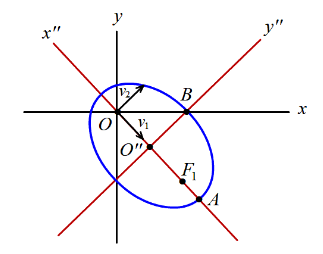
\includegraphics[width=\textwidth, height=\textheight, keepaspectratio]{images/ej3.png}
  \end{figure}
\end{frame}

\section{Bibliografía}

\begin{frame}{Bibliografía}
  \begin{itemize}
    \item \faGlobe\, Applications of Linear Algebra in Various Fields (Part-1): \url{https://www.researchgate.net/publication/356818396_Applications_of_Linear_Algebra_in_Various_Fields_Part-1}
    \item \faBook\, J. de Burgos. Álgebra lineal y geometría cartesiana. McGraw Hill 2a Ed. (2000)
    \item \faBook\, G. Farin, D. Hansford. Practical Linear Algebra: a geometry toolbox. A.K. Peters (2005).
  \end{itemize}
\end{frame}

% \begin{frame}[standout]
%   Gracias \\
% \end{frame}

\end{document}